%\documentstyle[epsf,twocolumn]{jarticle}       %LaTeX2.09仕様
\documentclass[twocolumn]{jarticle}     %pLaTeX2e仕様

%\usepackage[backend=bibtex, style=numeric]{biblatex}
%\addbibresource{sankou.bib}
%%%%%%%%%%%%%%%%%%%%%%%%%%%%%%%%%%%%%%%%%%%%%%%%%%%%%%%%%%%%%%
%%
%%  基本 バージョン
%%
%%%%%%%%%%%%%%%%%%%%%%%%%%%%%%%%%%%%%%%%%%%%%%%%%%%%%%%%%%%%%%%%
\setlength{\topmargin}{-45pt}
%\setlength{\oddsidemargin}{0cm}
\setlength{\oddsidemargin}{-7.5mm}
%\setlength{\evensidemargin}{0cm}
\setlength{\textheight}{24.1cm}
%setlength{\textheight}{25cm}
\setlength{\textwidth}{17.4cm}
%\setlength{\textwidth}{172mm}
\setlength{\columnsep}{11mm}

\setlength{\intextsep}{8pt}
\setlength{\textfloatsep}{8pt}
\setlength{\floatsep}{1pt}

\kanjiskip=.07zw plus.5pt minus.5pt



%【節がかわるごとに(1.1)(1.2) …(2.1)(2.2)と数式番号をつけるとき】
%\makeatletter
%\renewcommand{\theequation}{%
%\thesection.\arabic{equation}} %\@addtoreset{equation}{section}
%\makeatother

%\renewcommand{\arraystretch}{0.95} 行間の設定

\usepackage[dvipdfmx]{graphicx}   %pLaTeX2e仕様(\documentstyle ->\documentclass)
\usepackage[dvipdfmx]{color}
\usepackage{scalefnt}
\usepackage{bm}
\usepackage{here}
\usepackage{url}
\usepackage{amsmath}
\usepackage{amsfonts}
\usepackage[subrefformat=parens]{subcaption}
\captionsetup{compatibility=false}
%%%%%%%%%%%%%%%%%%%%%%%%%%%%%%%%%%%%%%%%%%%%%%%%%%%%%%%%
\usepackage{comment}
\usepackage{subcaption}
\usepackage{multirow}
\usepackage{nidanfloat}
%\usepackage[table,xcdraw]{xcolor}
\usepackage[dvipdfmx]{hyperref}

\usepackage[normalem]{ulem}
\useunder{\uline}{\ul}{}

\begin{document}

\twocolumn[
\noindent
\hspace{1em}

令和2年7月1日(水) ゼミ資料
\hfill
\ \ B4 高山 裕成

\vspace{2mm}
\hrule
\begin{center}
{\Large  進捗報告}
\end{center}
\hrule
\vspace{3mm}
]

% \footnotesize
\section{進捗}

\begin{itemize}
  \item 単文のマルチモーダル感情推定 (発表資料より抜粋しています)
\end{itemize}

\subsection{illustration2vec}
illustration2vec\cite{i2v} は, Masaki Saito と Yusuke Matsui らが提案した画像のベクトル化手法で, Danbooru と Safebooru から 100 万枚のイラストを用いて学習した事前学習済みモデルが公開されている. illustration2vec で扱った問題としてイラストに対する画像認識の難しさがあり, 既存の画像認識モデルのほとんどが ImageNet などを評価対象にしており, アニメや漫画といったイラストに対して評価を行っていなかったため, イラストのベクトル化手法に関してより良い期待が持てる手法である. 本稿では事前学習済みモデルを使って 4096 次元のコマ画像のベクトルを獲得する. 概要図を図\ref{fig:i2v} に示す.

\begin{figure*}[!bth]
  \begin{center}
    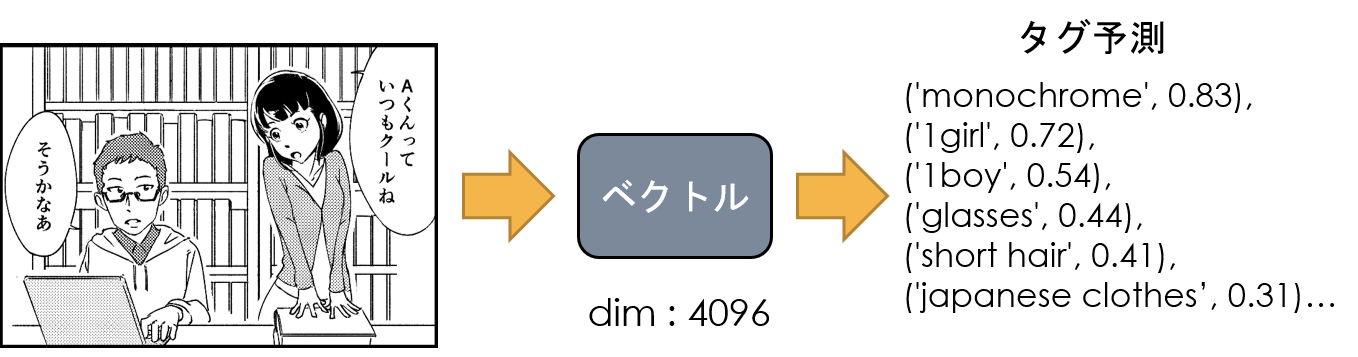
\includegraphics[scale=0.7]{i2v.png}
    \caption{i2v 概要図} %タイトルをつける
    \label{fig:i2v} %ラベルをつけ図の参照を可能にする
  \end{center}
\end{figure*}


\section{\small{実験 1 : 時系列を考慮しないセリフの感情推定}}
この実験では 1 つのセリフを入力し, 対応する感情ラベルを出力するような感情推定を行う. JUMAN++ \footnote{http://nlp.ist.i.kyoto-u.ac.jp/index.php?JUMAN++} によって分かち書きされたセリフを BERT への入力とし, 識別器としては 3 層 MLP を用いた. 表\ref{table:mlp_para}に MLP で用いたパラメータ, そして表\ref{table:ex_para}に学習で用いたパラメータを示す. 学習率は optuna によって最適なパラメータを探索した.

BERT の事前学習済みモデルの全ての重みを固定した場合 (BERT fixed) と最終層のパラメータだけをチューニングした場合 (BERT last layer) の 2 つの手法について感情推定を行い, 各タッチ・手法の結果について比較し, fine tuning の有用性を確かめることを目的とした.

表\ref{table:result_1}は各タッチについて, 評価用データの結果をまとめたものである.
表\ref{table:result_1}より, Accuracy に関しては差異はないが共にベースラインを超え, Recall, F1 値共に BERT fixed より BERT last layer の方が上回ったことから, fine tuning の有用性を確かめることができた.

\section{\small{実験 3 : 単文のマルチモーダル感情推定}}
実験 1 において, BERT から得た 768 次元のベクトルと, 入力したセリフが含まれているコマ全体の画像を illustration2vec に入力し, 得た 4096 次元のベクトルを concat した 4864 次元のベクトルを, 同様に 3 層 MLP に入力することでマルチモーダルな感情推定を行った. データセット整備の都合上, 少年漫画タッチ, 青年漫画タッチ, 萌えタッチについてのみ実験を行った.

表\ref{table:result_3}は 3 タッチについて, 評価用データの結果をまとめたものである. 比較として, 実験 1 における 3 タッチの結果も載せている.
表\ref{table:result_3}より, 実験 1 と比べ, Recall 以外の評価指標は下回ったが, 少年漫画タッチにおいては今回の実験を通して最も高い Recall と F1 値が出ており, マルチモーダルな感情推定を行う意味はあると推測できる.


\begin{table}[htb]
\caption{実験 1 MLP パラメータ}
\label{table:mlp_para}
\centering
\begin{tabular}{|c||c|c|}
\hline
& MLP \\ \hline
(in,hidden,out) & (768,30,2) \\ \hline
activation function & tanh \\ \hline
dropout rate & 0.5 \\ \hline
\end{tabular}
\end{table}

\begin{table}[htb]
\caption{学習パラメータ}
\label{table:ex_para}
\centering
\begin{tabular}{|c||c|c|}
\hline
& \multicolumn{2}{|c|}{実験 $1・2・3$} \\ \hline
epoch & \multicolumn{2}{|c|}{200}  \\ \hline
batch size & \multicolumn{2}{|c|}{16} \\ \hline
loss function & \multicolumn{2}{|c|}{Cross Entropy Loss} \\ \hline
optimizer & \multicolumn{2}{|c|}{Adam} \\ \hline
\end{tabular}
\end{table}

\begin{table*}[!b]
\begin{center}
\caption{実験 1 結果(評価用データ)}
\label{table:result_1}
\scalebox{0.66}{
\begin{tabular}{cccccccccccccccc|ccc}
\hline
\multirow{2}{*}{} & \multicolumn{3}{c}{ギャグ} & \multicolumn{3}{c}{少女漫画} & \multicolumn{3}{c}{少年漫画} & \multicolumn{3}{c}{青年漫画} & \multicolumn{3}{c|}{萌え系} & \multicolumn{3}{c}{5タッチ総合} \\
 & Acc & Recall & F1 & Acc & Recall & F1 & Acc & Recall & F1 & Acc & Recall & F1 & Acc & Recall & F1 & Acc & Recall & F1 \\ \hline
BERT fixed & 0.757 & 0.200 & 0.200 & 0.552 & 0.684 & 0.634 & 0.796 & 0.000 & 0.000 & 0.784 & 0.357 & 0.416 & 0.718 & 0.454 & 0.526 & 0.720 & 0.447 & 0.485 \\
BERT last layer & 0.818 & 0.200 & 0.250 & 0.641 & 0.710 & 0.692 & 0.781 & 0.000 & 0.000 & 0.800 & 0.500 & 0.518 & 0.578 & 0.500 & 0.448 & 0.723 & 0.489 & {\ul 0.510} \\ \hline
ベースライン & \multicolumn{1}{l}{0.848} & 0.000 & 0.000 & 0.432 & 0.000 & 0.000 & 0.812 & 0.000 & 0.000 & 0.784 & 0.000 & 0.000 & 0.656 & 0.000 & 0.000 & 0.705 & 0.000 & 0.000
\end{tabular}
}
\end{center}
\end{table*}


\begin{table*}[!b]
\begin{center}
\caption{実験 3 結果(評価用データ)}
\label{table:result_3}
\scalebox{0.68}{
\begin{tabular}{cccccccccccccccc|ccc}
\hline
\multirow{2}{*}{} & \multicolumn{3}{c}{ギャグ} & \multicolumn{3}{c}{少女漫画} & \multicolumn{3}{c}{少年漫画} & \multicolumn{3}{c}{青年漫画} & \multicolumn{3}{c|}{萌え系} & \multicolumn{3}{c}{3タッチ総合} \\
 & Acc & Recall & F1 & Acc & Recall & F1 & Acc & Recall & F1 & Acc & Recall & F1 & Acc & Recall & F1 & Acc & Recall & F1 \\ \hline
実験 1 fixed & - & - & - & - & - & - & 0.796 & 0.000 & 0.000 & 0.784 & 0.357 & 0.416 & 0.718 & 0.454 & 0.526 & 0.766 & 0.312 & 0.400 \\
実験 1 last layer & - & - & - & - & - & - & 0.781 & 0.000 & 0.000 & 0.800 & 0.500 & 0.518 & 0.578 & 0.500 & 0.448 & 0.720 & 0.375 & 0.400 \\ \hline
実験 3 & - & - & - & - & - & - & 0.531 & 0.500 & 0.285 & 0.784 & 0.500 & 0.500 & 0.562 & 0.363 & 0.363 & 0.626 & 0.437 & 0.368 \\ \hline
ベースライン & - & - & - & - & - & - & 0.812 & 0.000 & 0.000 & 0.784 & 0.000 & 0.000 & 0.656 & 0.000 & 0.000 & 0.751 & 0.000 & 0.000
\end{tabular}
}
\end{center}
\end{table*}

\bibliographystyle{unsrt}
\bibliography{sankou}


\end{document}
